\documentclass[10pt, conference]{IEEEtran}
\hyphenation{op-tical net-works semi-conduc-tor}
\usepackage{graphicx}
\usepackage{fancyhdr}
\usepackage{url}
\usepackage{amsmath}
\usepackage{listings}
\usepackage{algorithm}
\usepackage{algorithmic}
\usepackage{lipsum}
\usepackage{bookmark}
\usepackage[normalem]{ulem}
\useunder{\uline}{\ul}{}

\pagestyle{fancy}
\fancyhf{}
\lhead{\textsc{ELEN4020}}
\rhead{\textsc{Laboratory Exercise No 1}}
\rfoot{Page \thepage\ }


\begin{document}
\begin{titlepage}
\newcommand{\HRule}{\rule{\linewidth}{0.5mm}} % Defines a new command for the horizontal lines, change thickness here

\center % Center everything on the page
 
%----------------------------------------------------------------------------------------
%	HEADING SECTIONS
%----------------------------------------------------------------------------------------

\textsc{\LARGE University of Witwatersrand}\\[1.5cm] % Name of your university/college
%----------------------------------------------------------------------------------------
%	LOGO SECTION
%----------------------------------------------------------------------------------------


\includegraphics[scale=0.25]{Wits.png}% Include a department/university logo - this will require the graphicx package
 
 
%----------------------------------------------------------------------------------------
\textsc{\Large ELEN4020}\\[0.5cm] % Major heading such as course name
\textsc{\large Data Intensive Computing In Data Science}\\[0.5cm] % Minor heading such as course title



%----------------------------------------------------------------------------------------
%	TITLE SECTION
%----------------------------------------------------------------------------------------

\HRule \\[0.4cm]
{ \huge \bfseries Laboratory Exercise 1}\\[0.4cm] % Title of your document
\HRule \\[1.5cm]
 
%----------------------------------------------------------------------------------------
%	AUTHOR SECTION
%----------------------------------------------------------------------------------------

\begin{minipage}{0.4\textwidth}
\begin{flushleft} \large
	\emph{Authors:}\\
	\textsc{Kishan Narotam - 717 931\\Jesal Chana - 603 177} 
\end{flushleft}
\end{minipage}
~
\begin{minipage}{0.4\textwidth}
\begin{flushright} \large
	\emph{Authors:} \\
	\textsc{Syed Hussain - 600 524\\Yusuf Ally - 604 973} 
\end{flushright}
\end{minipage}\\[2cm]


%----------------------------------------------------------------------------------------
%	DATE SECTION
%----------------------------------------------------------------------------------------

{\large 23\textsuperscript{rd} February 2018}\\[2cm] % Date, change the \today to a set date if you want to be precise

%-------------------------------------------------------------------------------------
%----------------------------------------------------------------------------------------

\vfill % Fill the rest of the page with whitespace

\end{titlepage}
%----------------------------------------------------------------------------------------

%----------------------------------------------------------------------------------------
%	MAIN BODY OF REPORT
%----------------------------------------------------------------------------------------

\section{Problem Description}
\label{Problem Description}
A \emph{K}-dimensional integer array, represented as $A[N_0][N_1]...[N_{K-1}]$, must be created for different values of \emph{K}. The integer array is bounded by $N_0, N_1,...,N_{K-1}$, and once created, the array must undergo three procedures which are as follows:
\begin{enumerate}
\item Initialize all elements in the array to be zeroes
\item Set 10\% of all elements in the array uniformly to 1's
\item In a random fashion across all dimensions in the array:
	\begin{enumerate}
	\item Choose 5\% of the elements
	\item Print the coordinate indices of the elements
	\item Print the value of the element at the chosen cell.
	\end{enumerate}
\end{enumerate}

Four integer arrays must be created, each with various dimension size as well as array size. For each of these arrays, the three procedures must be called, however it must be completed as if the number of dimensions in the array are not static.

\section{Background}
\label{Background}
An array is defined as a data structure that contains a group of elements, in the case of this problem the elements are integers~\cite{Array Def}. An array can have multiple dimensions, for example an array with one dimension is regarded as a row, whereas an array with two dimensions is regarded as a matrix with a row and a column. However as the dimensions of the matrix reach three or more, the array has a new coordinate property known as depth/page~\cite{Eli, Mathworks}. Figure~\ref{DimArray} in Appendix~\ref{Diagrams} is a representation of a 3-dimensional array with the coordinate properties. As the dimensions increase it becomes more difficult to represent these arrays in a graphical representation.


\subsection{Memory Allocation}
\label{Memory Allocation}
The memory and layout of a \emph{K}-dimensional array could be allocated in multiple ways. Two of the most common ways of this memory layout are row-major order or column-major order. 

In a 2D array, the row-major order layout would put the first row in contiguous memory, the second row would follow, and so on. Similarly, for column-major order layout, the first column would be in contiguous memory, the second column would follow and so on~\cite{Eli}.

In a 3D array, using the dimensions of row, column and depth/page, Figure~\ref{3DArray} in Appendix~\ref{Diagrams} shows how a 3-dimensional array memory is allocated and how the layout is presented in row-major order~\cite{Eli}.

In order to calculate the memory location of an element from its respective index in the array, the following formulae can be used for row-major order and column-major order respectively for a \emph{K}-dimensional array.


\begin{equation}
\label{eqn1}
\begin{split}
offset &= n_K + N_K \cdot (n_{K-1} +N_{K-1} \cdot (n_{K-2} +N_{K-2} \cdot\\& (...+N_2n_1)...) )\\
&= \sum_{i=1}^{K} \bigg(\prod_{j=i+1}^{K} N_j \bigg) n_i
\end{split}
\end{equation}

\begin{equation}
\label{eqn2}
\begin{split}
offset &= n_1 + N_1 \cdot (n_2 +N_2 \cdot (n_3 +N_3 \cdot (...+N_{K-1}n_K)...) )\\
	&= \sum_{i=1}^{K} \bigg(\prod_{j=1}^{i-1} N_j \bigg) n_i
\end{split}
\end{equation}

\section{Function Descriptions}
\label{Function Description}
\subsection{\texttt{main}}
This is the function that is responsible for calling the subsequent functions. The user is given two options, whether to enter an array of any dimension and any size and to perform the three procedures or to perform the three procedures of the predefined arrays presented in Section~\ref{Problem Description}.

\subsection{\texttt{allocateArray}}
This function has two main responsibilities : to dynamically allocate the desired array, and to then call the three procedures that execute on the array.
This function takes as inputs the initializer array (\texttt{iniArray[]}), and the number of dimensions.

\subsubsection{Dynamic memory allocation}
The array is generated using \texttt{malloc}, which allocates a contiguous memory block. The size of the block is determined by the number of elements in the array and the number of bytes per element.
\subsubsection{Calling procedures}
Once the array has been generated, the three procedures are called in succession.

\subsection{\texttt{procedureOne}}
This procedure sets every element in the array to zero. It takes as inputs the array, and the number of elements in the array (in order to know how many elements it should step through).

\subsection{\texttt{procedureTwo}}
This procedure sets the first 10\% of elements of the array to one. Like \texttt{procedureOne} it takes as inputs the array and the number of elements in the array. Variable \texttt{tenPercentElements} is the value of 10\% of elements of the array, and is used to determine whether an element should be set to one.

\subsection{\texttt{procedureThree}}
This procedure randomly chooses 5\% of elements in the array and prints the corresponding value and coordinate indices of these elements.
\subsubsection{Random coordinate generation}
The initialized array is in the form  \texttt{int iniArray[] = } $\{N_0 , N_1 , ... , N_{K-1} \}$, where $K$ is the array dimension and $N_0 , N_1 , ...$ are the sizes of each dimension. For example, \texttt{int iniArray[] = } $\{3 , 3 \}$ creates a 2D $(3 X 3)$ array.\newline\newline

A random coordinate for all $K$ indexes is generated using \texttt{$rand()\%N_K$}, where \texttt{$\%N_K$} bounds each coordinate index. This bounding ensures a valid coordinate is created every time. Each coordinate is then stored in  \texttt{coordinate\_array}.
\subsubsection{Coordinate mapping}
The randomly generated coordinate is now mapped to its 1D linear array index. This is done using the row major order indexing equation (lines 150-156). The corresponding value is obtained using this index. The coordinate and value is then printed, for 5\% of elements in the array.

\section{Pseudo Code}
\label{Pseudo Code}
The pseudo code for the entire program is seen in Appendix~\ref{Pseudo Appendix}. Although written in one file, each function is split up into their own algorithms to better understand the pseudo code of each. Algorithm~\ref{Main} in Appendix~\ref{Pseudo Appendix} is the pseudo code for the \texttt{main} function and Algorithm~\ref{allocateArray} in Appendix~\ref{Pseudo Appendix} is the pseudo code for the \texttt{allocateArray} void function. Algorithms~\ref{procedureOne},~\ref{procedureTwo},~\ref{procedureThree} in Appendix~\ref{Pseudo Appendix}, are the pseudo codes for the first, second and third procedures respectively.

\section{Final Code and Output}
\label{Final Code and Output}
The final program was coded in C on an Ubuntu system and compiled using a custom makefile. The program was tested using \emph{K}-dimensional arrays of different size to ensure it works as desired. These outputs can be seen in Figures~\ref{Result2D},~\ref{Result3D},~\ref{Result4D}, and~\ref{Result5D} in Appendix~\ref{Output}. The four given arrays mentioned in section~\ref{Problem Description} are tested in the program and yield the relevant results.


\section{Conclusion}
\label{Conclusion}
A method was created to step through the elements of multiple arrays which varied in size and dimensions. The program yielded relevant results and was done so in a general way, i.e. the number of dimensions in the array are dynamic, as opposed to a nested loop. The coding was done in C on an Ubuntu operating system and was executed using a makefile in the command line prompt.


\begin{thebibliography}{}

\bibitem{Array Def}
Christensson, P; \emph{Array Definition}; \url{https://eli.thegreenplace.net/2015/memory-layout-of-multi-dimensional-arrays}; Last Accessed: 21/02/2018

\bibitem{Eli}
Bendersky, E; \emph{Memory layout of multi-dimensional arrays - Eli Bendersky's website}; \url{https://eli.thegreenplace.net/2015/memory-layout-of-multi-dimensional-arrays}; Last Accessed: 21/02/2018

\bibitem{Mathworks}
Mathworks; \emph{Multidimensional Arrays - MATLAB \& Simulink}; \url{https://www.mathworks.com/help/matlab/math/multidimensional-arrays.html}; Last Accessed: 21/02/2018

\end{thebibliography}

\onecolumn
\center
\begin{appendices}
\section{Diagrams}
\label{Diagrams}

\begin{figure}[h!]
\renewcommand{\thefigure}{\arabic{figure}}
\centering
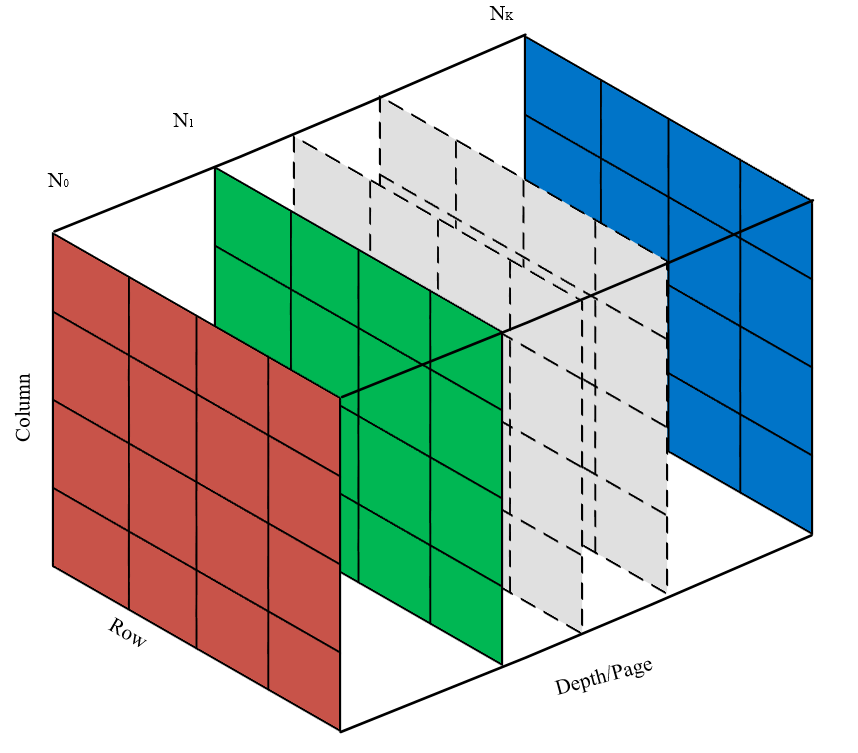
\includegraphics[scale=0.4]{DimensionalArray.png}
\caption{Representation of a \emph{3}-dimensional array}
\label{DimArray}
\end{figure}

\begin{figure}[h!]
\renewcommand{\thefigure}{\arabic{figure}}
\centering
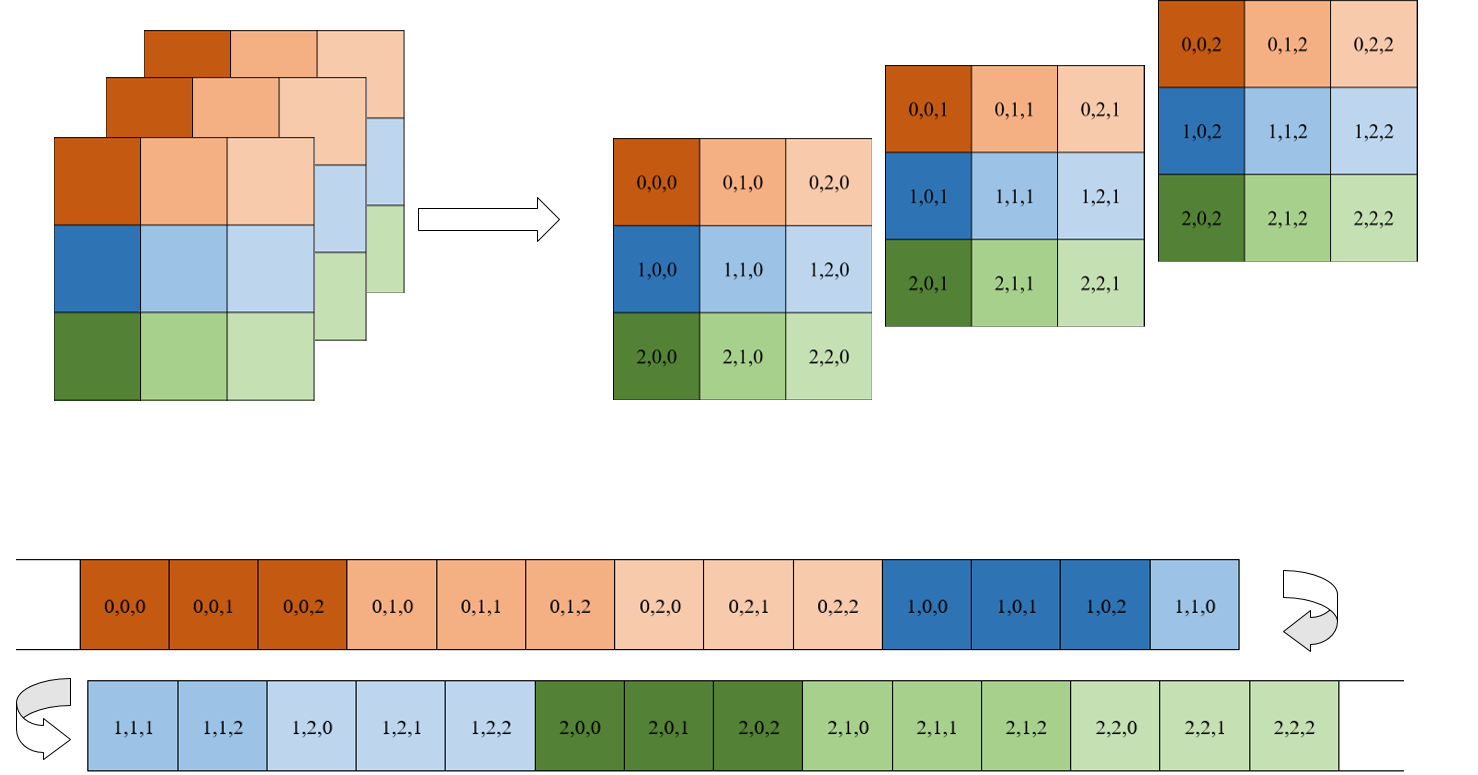
\includegraphics[scale=0.5]{MemoryAlloc.png}
\caption{Memory allocation of a 3-dimensional in row-major order~\cite{Eli}}
\label{3DArray}
\end{figure}

\onecolumn
\section{Pseudo Code}
\label{Pseudo Appendix}

\begin{algorithm}[h!]
\caption{\texttt{main} Function}
\label{Main}
\begin{algorithmic} 

\STATE $srand(time(NULL))$
\STATE $Dimension$
\STATE $mode$
\STATE
\STATE Display ``Press 1 to run or 2 to input an array''
\STATE $mode \leftarrow$ User input
\IF{$mode = 2$}
	\STATE Display ``Enter array dimension: ''
	\STATE $Dimension \leftarrow$ User input
	\STATE $userArray[Dimension]$
	\STATE Display ``Enter the size of each dimension: ''
	\FOR{$i = 0$ to $Dimensions$}
		\STATE $userArray[i] \leftarrow$ User input
	\ENDFOR
	\STATE $allocateArray(userArray, Dimension)$
\ENDIF
\STATE
\IF{$mode = 1$}
	\STATE $arrayInitializer1[\ ] \leftarrow (100, 100)$
	\STATE $Dimension \leftarrow sizeof(arrayInitializer1)/sizeof(int)$
	\STATE $allocateArray(arrayInitializer1, Dimension)$
	\STATE
	\STATE $arrayInitializer2[\ ] \leftarrow (100, 100, 100)$
	\STATE $Dimension \leftarrow sizeof(arrayInitializer2)/sizeof(int)$
	\STATE $allocateArray(arrayInitializer2, Dimension)$
	\STATE
	\STATE $arrayInitializer3[\ ] \leftarrow (50, 50, 50, 50)$
	\STATE $Dimension \leftarrow sizeof(arrayInitializer3)/sizeof(int)$
	\STATE $allocateArray(arrayInitializer3, Dimension)$
	\STATE
	\STATE $arrayInitializer4[\ ] \leftarrow (20, 20, 20, 20, 20)$
	\STATE $Dimension \leftarrow sizeof(arrayInitializer4)/sizeof(int)$
	\STATE $allocateArray(arrayInitializer4, Dimension)$
\ENDIF

\end{algorithmic}
\end{algorithm}

\begin{algorithm}[h!]
\caption{\texttt{allocateArray} Function}
\label{allocateArray}
\begin{algorithmic} 

\STATE \textbf{Input:} $iniArray[\ ]$ and $dimension$
\STATE
\STATE $num\_elements \leftarrow 1$
\FOR{$i = 0$ to $dimension$}
	\STATE $num\_elements \leftarrow num\_elements * iniArray[i]$
\ENDFOR
\STATE refToInteger $array$
\STATE $array \leftarrow$ refToInteger $malloc(sizeof($refToInteger $num\_elements))$
\STATE Display ``Dimensions $dimensions$, Elements $num\_elements$''
\STATE
\IF{$array\leftarrow NULL$}
	\STATE Display ``malloc failed''
	\STATE $exit(1)$
\ENDIF
\STATE
\FOR{$i = 0$ to  $num\_elements$}
	\STATE $array[i] \leftarrow i$
\ENDFOR
\STATE $procedureOne(array, num\_elements)$
\STATE $procedureTwo(array, num\_elements)$
\STATE $procedureThree(array, iniArray, num\_elements, dimension)$

\end{algorithmic}
\end{algorithm}

\begin{algorithm}[h!]
\caption{\texttt{procedureOne} Function}
\label{procedureOne}
\begin{algorithmic} 

\STATE \textbf{Input:} $arr[\ ]$ and $numElements$
\STATE
\STATE Display ``Procedure 1: ''
\FOR{$i = 0$ to $numElements$}
	\STATE $arr[i] \leftarrow 0$
\ENDFOR
\STATE Display ``...Executed procedure 1...''

\end{algorithmic}
\end{algorithm}


\begin{algorithm}[h!]
\caption{\texttt{procedureTwo} Function}
\label{procedureTwo}
\begin{algorithmic} 

\STATE \textbf{Input:} $arr[\ ]$ and $numElements$
\STATE
\STATE Display ``Procedure 2: ''
\STATE $tenPercentElements \leftarrow numElements/10$
\FOR{$i = 0$ to $numElements$}
	\IF{$i < tenPercentElements$}
		\STATE $arr[i] \leftarrow 1$
	\ENDIF
\ENDFOR
\STATE Display ``...Executed procedure 2...''

\end{algorithmic}
\end{algorithm}

\begin{algorithm}[h!]
\caption{\texttt{procedureThree} Function}
\label{procedureThree}
\begin{algorithmic} 

\STATE \textbf{Input:} $arr[\ ]$, $arr2[\ ]$, $numberElements$, $dimensions$
\STATE
\STATE Display ``Procedure 3: ''
\STATE $fivePercentElements \leftarrow numberElements*5/100$
\FOR{$a = 0$ to $fivePercenElements$}
	\STATE refToInteger $coordinate\_array$
	\STATE $array \leftarrow$ refToInteger $malloc(sizeof($refToInteger $dimension))$	
	\STATE Display ``Coordinate = (''
	\FOR{$i = 0$ to $dimension$}
		\STATE $coordinate\_array[i] \leftarrow rand()\%arr2[i]$
		\STATE Display $coordinat\_array[i]$
		\IF{$i < dimension -1$}
			\STATE Display ``,''
		\ENDIF
	\ENDFOR
	\STATE Display ``)''
	\STATE $product \leftarrow 1$
	\STATE $index \leftarrow 0$
	\STATE $product2 \leftarrow 1$
	\FOR{$i = 0$ to $dimension-1$}
		\STATE $product \leftarrow 1$
		\FOR{$j = i+1$ to including $dimension-1$}
			\STATE $product \leftarrow product * arr2[j]$
		\ENDFOR
		\STATE $product2 \leftarrow product*coordinate\_array[i]$
		\STATE $index \leftarrow index + product2$
	\ENDFOR
	\STATE Display `` ; Value = '' $arr[index]$
\ENDFOR
\STATE Display ``...Executed procedure 3...''

\end{algorithmic}
\end{algorithm}



\onecolumn
\center
\section{Output}
\label{Output}

\begin{figure}[h!]
\renewcommand{\thefigure}{\arabic{figure}}
\centering
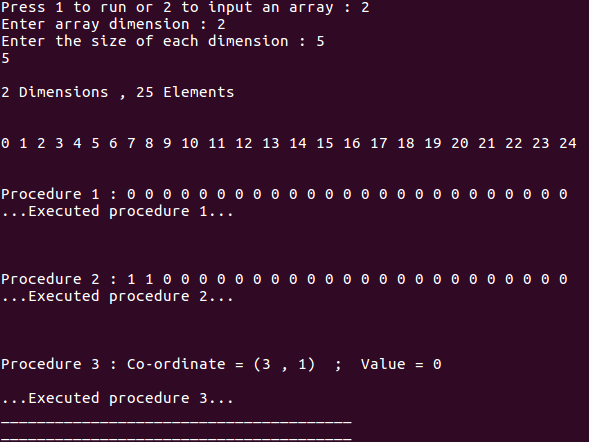
\includegraphics[scale=0.4]{Result2D.png}
\caption{Output result of a 2-Dimensional Array of size 5, i.e. \texttt{Array[5][5]} }
\label{Result2D}
\end{figure}

\begin{figure}[h!]
\renewcommand{\thefigure}{\arabic{figure}}
\centering
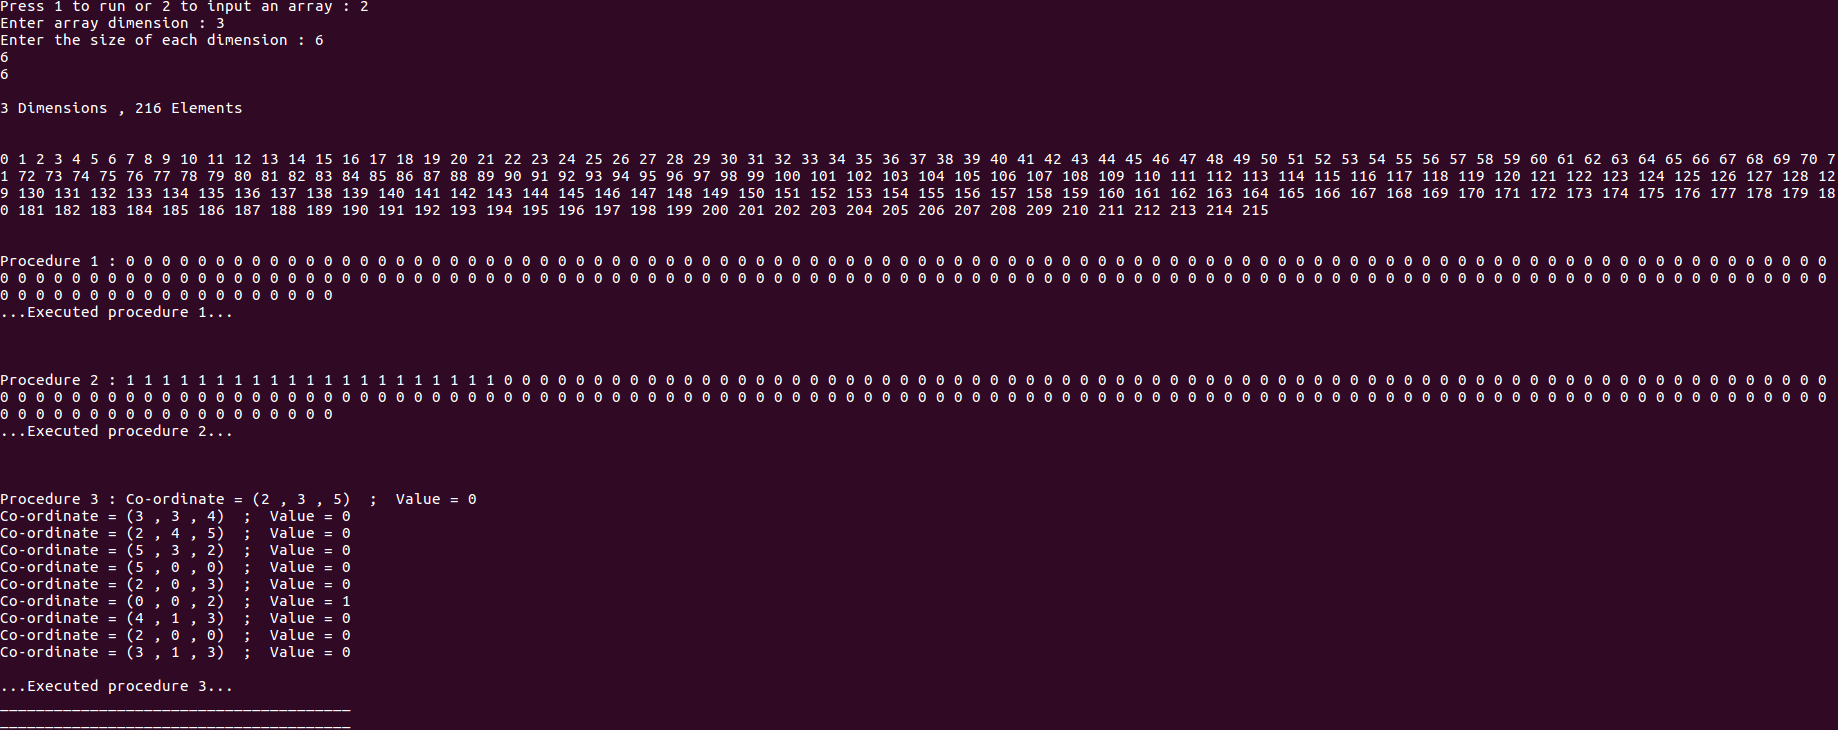
\includegraphics[scale=0.3]{Result3D.png}
\caption{Output result of a 3-Dimensional Array of size 6, i.e. \texttt{Array[6][6][6]} }
\label{Result3D}
\end{figure}

\begin{figure}[h!]
\renewcommand{\thefigure}{\arabic{figure}}
\centering
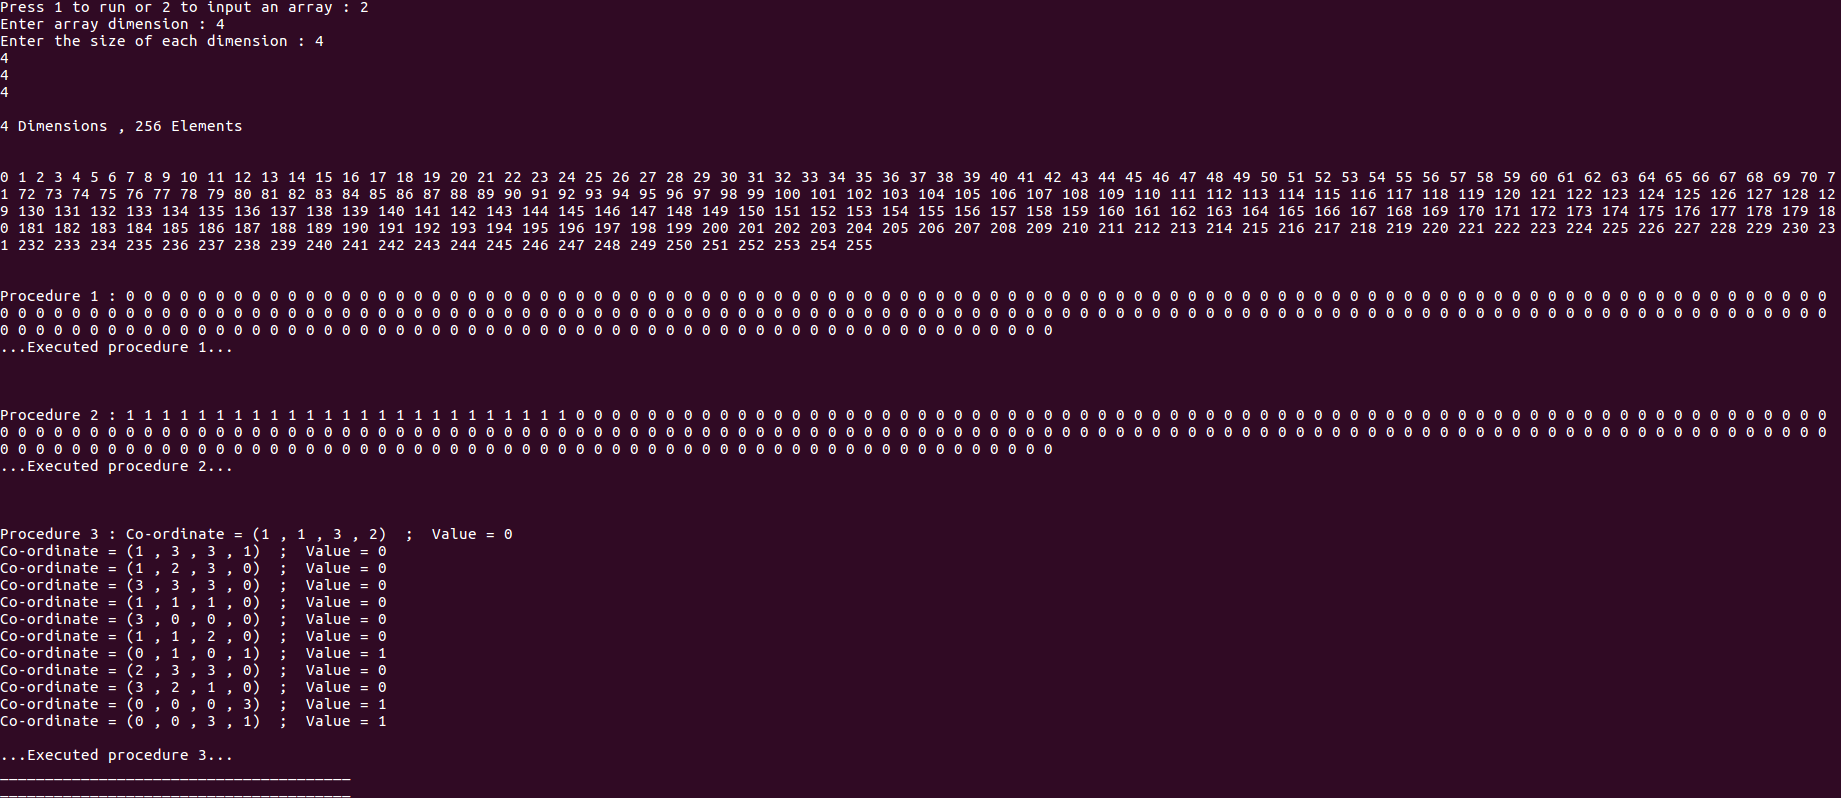
\includegraphics[scale=0.3]{Result4D.png}
\caption{Output result of a 4-Dimensional Array of size 4, i.e. \texttt{Array[4][4][4][4]} }
\label{Result4D}
\end{figure}

\begin{figure}[h!]
\renewcommand{\thefigure}{\arabic{figure}}
\centering
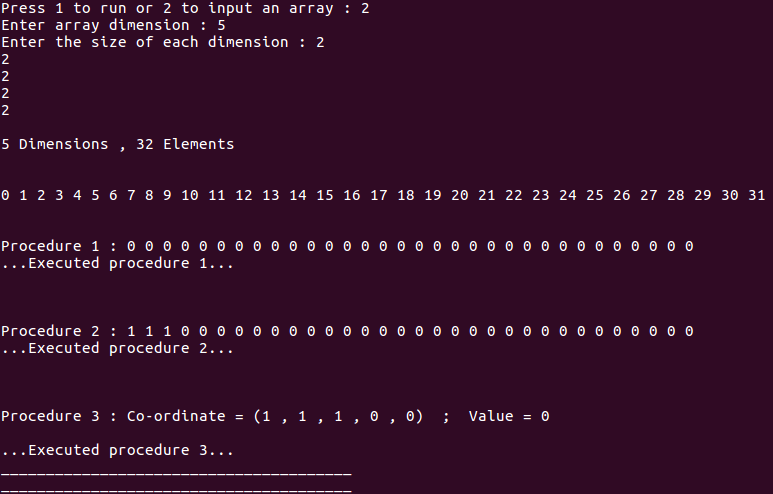
\includegraphics[scale=0.5]{Result5D.png}
\caption{Output result of a 5-Dimensional Array of size 2, i.e. \texttt{Array[2][2][2][2][2]} }
\label{Result5D}
\end{figure}

\end{appendices}




% that's all folks
\end{document}


